\documentclass[tikz,border=10pt]{standalone}
\usepackage{amsmath}
\usepackage{amssymb}
\usepackage{tikz}
\usetikzlibrary{arrows.meta,calc,decorations.pathreplacing,patterns,shapes.geometric,positioning,shadings}

\definecolor{filmblue}{HTML}{CFE4F0}
\definecolor{rayred}{HTML}{C0392B}
\definecolor{rayblue}{HTML}{2B6CB0}
\definecolor{rayyellow}{HTML}{D4A017}

\begin{document}
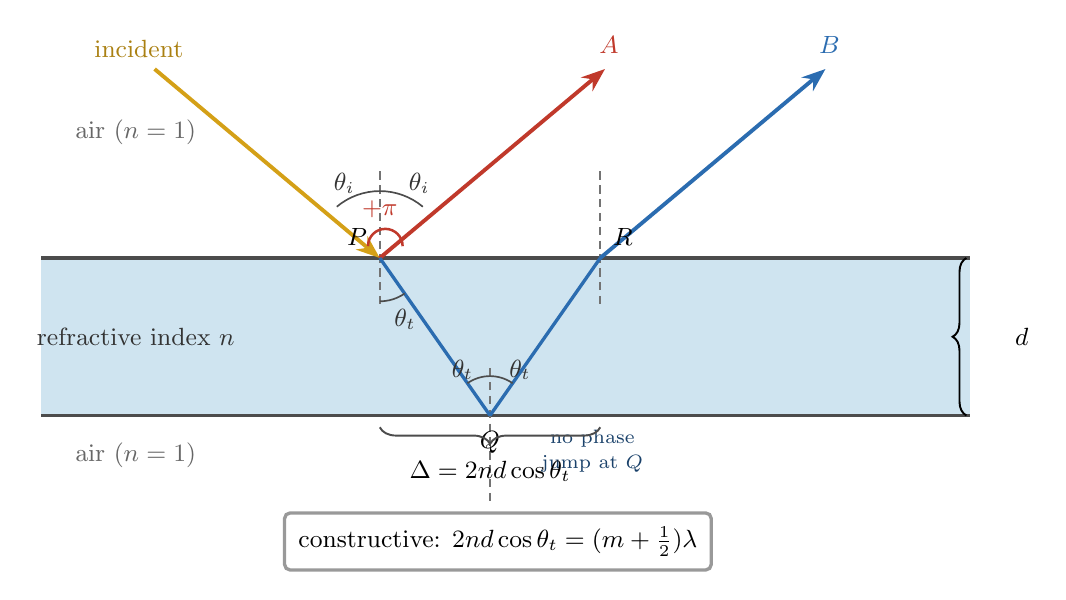
\begin{tikzpicture}[line width=1.2pt, >=Stealth, font=\small]

  % Film boundaries
  \def\xL{-5.8}
  \def\xR{6.0}
  \def\yTop{0}
  \def\yBot{-2.0}

  % Film fill
  \fill[filmblue] (\xL,\yTop) rectangle (\xR,\yBot);

  % Film top & bottom surfaces
  \draw[black!70] (\xL,\yTop) -- (\xR,\yTop);
  \draw[black!70] (\xL,\yBot) -- (\xR,\yBot);

  % Key points
  % Incident angle theta_i (from vertical), refracted angle theta_t
  % Choose angles so that tan(theta_i) > tan(theta_t): theta_i = 50 deg, theta_t ~ 35 deg (gives n ~ 1.34)
  % P on top surface
  \coordinate (P) at (-1.5, 0);
  % Q on bottom surface, directly below midpoint of P-R
  % Refracted ray from P goes down-right at angle theta_t=35 from vertical
  % Horizontal offset from P to Q: (yTop-yBot)*tan(35) = 2*0.7002 = 1.4004
  \coordinate (Q) at ($(P) + (1.4, -2.0)$);
  % R is reflection point on top surface; by symmetry, horizontal dist Q->R equals P->Q
  \coordinate (R) at ($(Q) + (1.4, 2.0)$);

  % Incident ray: comes from upper-left, angle theta_i=50 deg from vertical
  % direction into P from upper-left: from (P) + (-2*tan50, +2) roughly
  % tan50 ~ 1.1918
  \coordinate (Iin) at ($(P) + (-2.86, 2.4)$);
  % Reflected ray A from P at angle 50 deg from vertical, going upper-right
  \coordinate (Aout) at ($(P) + (2.86, 2.4)$);
  % Transmitted ray B exits at R at angle 50 deg from vertical (same as incident), upper-right
  \coordinate (Bout) at ($(R) + (2.86, 2.4)$);

  % --- Normal lines at P, Q, R (dashed) ---
  \draw[densely dashed, black!55, line width=0.6pt] ($(P)+(0,1.1)$) -- ($(P)+(0,-0.6)$);
  \draw[densely dashed, black!55, line width=0.6pt] ($(Q)+(0,0.6)$) -- ($(Q)+(0,-1.1)$);
  \draw[densely dashed, black!55, line width=0.6pt] ($(R)+(0,1.1)$) -- ($(R)+(0,-0.6)$);

  % --- Incident ray (white/yellow) ---
  \draw[rayyellow, -{Stealth[length=3mm]}, line width=1.4pt] (Iin) -- (P);
  \node[rayyellow!80!black] at ($(Iin)+(-0.2,0.25)$) {incident};

  % --- Reflected ray A (red) from P ---
  \draw[rayred, -{Stealth[length=3mm]}, line width=1.4pt] (P) -- (Aout);
  \node[rayred] at ($(Aout)+(0.05,0.3)$) {$A$};

  % --- Refracted ray P -> Q inside film ---
  \draw[rayblue, line width=1.2pt] (P) -- (Q);
  % --- Reflection at Q, Q -> R inside film ---
  \draw[rayblue, line width=1.2pt] (Q) -- (R);
  % --- Refracted ray exiting at R (ray B out) ---
  \draw[rayblue, -{Stealth[length=3mm]}, line width=1.4pt] (R) -- (Bout);
  \node[rayblue] at ($(Bout)+(0.05,0.3)$) {$B$};

  % --- Angles ---
  % theta_i at P (between normal and incident, on the left)
  \draw[black!70, line width=0.6pt] ($(P)+(0,0.85)$) arc[start angle=90, end angle=130, radius=0.85];
  \node[black!80] at ($(P)+(-0.45,0.95)$) {$\theta_i$};
  % reflection angle theta_i at P (right side, to Aout)
  \draw[black!70, line width=0.6pt] ($(P)+(0,0.85)$) arc[start angle=90, end angle=50, radius=0.85];
  \node[black!80] at ($(P)+(0.5,0.95)$) {$\theta_i$};
  % theta_t at P (inside film, below normal, to Q)
  \draw[black!70, line width=0.6pt] ($(P)+(0,-0.55)$) arc[start angle=-90, end angle=-55, radius=0.55];
  \node[black!80] at ($(P)+(0.32,-0.78)$) {$\theta_t$};
  % theta_t at Q (incoming from upper-left, and outgoing to upper-right, around upward normal)
  \draw[black!70, line width=0.6pt] ($(Q)+(0,0.5)$) arc[start angle=90, end angle=125, radius=0.5];
  \node[black!80] at ($(Q)+(-0.35,0.58)$) {$\theta_t$};
  \draw[black!70, line width=0.6pt] ($(Q)+(0,0.5)$) arc[start angle=90, end angle=55, radius=0.5];
  \node[black!80] at ($(Q)+(0.38,0.58)$) {$\theta_t$};

  % --- Point labels P, Q, R ---
  \node[above left=1pt of P, black] {$P$};
  \node[below=2pt of Q, black] {$Q$};
  \node[above right=1pt of R, black] {$R$};

  % --- Film labels: n, d ---
  \node[black!80] at (-4.6, -1.0) {refractive index $n$};
  % Thickness brace on right side
  \draw[decorate, decoration={brace, amplitude=5pt, mirror}, line width=0.7pt]
    ($(\xR, \yTop)+(-0.05,0)$) -- ($(\xR, \yBot)+(-0.05,0)$)
    node[midway, xshift=20pt, black] {$d$};

  % Air labels
  \node[black!60] at (-4.6, 1.6) {air ($n=1$)};
  \node[black!60] at (-4.6, -2.5) {air ($n=1$)};

  % --- pi phase jump at P (small semicircle above P on reflected side) ---
  % Small half-circle arrow indicating inversion
  \draw[rayred, line width=0.9pt] ($(P)+(-0.15,0.15)$) arc[start angle=180, end angle=0, radius=0.22];
  \node[rayred] at ($(P)+(0,0.62)$) {$+\pi$};

  % --- "no jump" at Q ---
  \node[rayblue!60!black, align=center] at ($(Q)+(1.3,-0.45)$) {\scriptsize no phase\\[-2pt]\scriptsize jump at $Q$};

  % --- Optical path difference bracket below film, under P-Q-R ---
  \draw[decorate, decoration={brace, amplitude=6pt, mirror}, line width=0.7pt, black!70]
    ($(P)+(0,-2.15)$) -- ($(R)+(0,-2.15)$)
    node[midway, yshift=-16pt, black] {$\Delta = 2nd\cos\theta_t$};

  % --- Constructive-interference condition box ---
  \node[draw=black!40, rounded corners=2pt, fill=white, inner sep=5pt] at (0,-3.6)
    {constructive: $2nd\cos\theta_t = (m+\tfrac12)\lambda$};

\end{tikzpicture}
\end{document}
